\chapter{Introduction} \label{chap:intro}

\paragraph{Motivation:}
Over the last decade, Software development had a tremendous impact with increasing customer demand and requirements \cite{article:swdemand:ahmed}. 
So, the developers have come up with different techniques to meet this requirement criteria. 
Similarly, increasing product complexity and ambiguity have a significant impact on software development. 
Early user feedback from potential customers in the industry is crucial for creating successful software products because of the growing market uncertainties, and consumers' desire to receive integrated solutions to their issues rather than unique software developments \cite{misc:businessmodels:teece}.
With the increasing complexity of products, it becomes challenging to determine user requirements.
Different people can have overlapping or contradicting opinions. 
And to reduce these risks, there has to be early detection of the user's needs and requirements. 
Giving users a ``partially functioning'' system is the most excellent method to determine their requirements \cite{journal:prototyping:davis}.
This ensures that the developers with high uncertainties in the early product development can validate by testing the underlying assumptions \cite{misc:lean:steve}.
Developers can use this feedback to validate the most critical assumptions about the software product. 
This validation can be used to decide whether to add, remove or update a feature \cite{article:experiments:lindgren}. 
This process is called \texttt{Continuous Experimentation (CE)}.
There has been an increase in interest in the types of experimentation that can take place in product development. 
Fabijan et al. \cite{article:controlled:experiements} have shown the benefits of continuous experiments in many use cases with incremental product improvement. 
In CE, the product owner designs different software variants (E.g., Different Subscription fees for registration) of the product, and the developer integrates these variants and assigns them to a distinct group of users. The variant with better results as per some evaluation criteria (more number of user registrations) is deployed for the entire set of users.
So, an experiment can be valuable when it solves real-world problems.
Hence, for experiments to be successful, they should offer one or more solutions that will benefit users.

\paragraph{Problem 1:} The developers are responsible for creating the experiments, and the product owners give the ideas and feedback to the developers.
The main problem is integrating the product owners and the non-developers into the development process to bridge the gap between the developers and non-developers.

\paragraph{Problem 2:} The process of creating experiments and testing their variants is usually not systematically arranged, creating anomalies that give rise to unsuccessful experiments. (Use design principles)

\paragraph{Problem 3:} In a small-scale company containing a few users, it is not easy to do experiments and get conclusive feedback on the ``winner'' variant. 
Because, with a small amount of data, it is impossible to prove one of the variants outperforms the others statistically.

\paragraph{Problem 4:} Most often, the software application collects data from the experiments, and not all the data is used in the analysis phase reducing the software applications to improve based on customer feedback. (Use Data-driven development)

\paragraph{Research Approach:} 
To solve the first problem, the developers focus more on automating the software code rather than coding everything stated in the product requirements \cite{article:prototyping:hoffnagle}.
This approach is formally known as a \texttt{Low-code} approach.
So, this approach helps to have a UI interface for the non-developers to understand and develop the software products \cite{paper:lowcode:khorram}.
One approach to support the product owners in developing the variants is UI Prototyping. 
UI prototyping creates new UI variants using predefined UI elements (E.g., Drag and drop the UI elements into the screen). 
This helps product owners to be creative and innovative because it gives them visual feedback.
So, if UI prototypes are developed in a low-code technique, they would be lightweight software that helps the product owner develop various prototypes and conduct experiments on the users.
According to Cabot et al. \cite{paper:lowcode:cabot}, the low-code has become more accessible for Model-driven development. 
Similarly, while creating prototyping, the software should have connections between the screens (E.g., clicking on a button should go to the next screen), and this logic can be achieved using Models.
Models are used broadly in prototyping because a model represents or describes the aspects of the systems that cannot be described adequately in a system of interest \cite{paper:prototyping:luqi}.
Moderately accurate models can be created using an iterative approach in software development by getting continuous feedback from the users.

To solve the \texttt{second} problem, a design science research (DSR) study should be conducted to obtain some Design Principles (DPs) defined for the whole process of experimentation \cite{paper:designprinciple:vk}. 
Here, DPs capture and codify that knowledge by focussing on the implementer, the aim, the user, the context, the mechanism, the enactors, and the rationale \cite{paper:designprinciple:gregor}. 
The DPs explain the design information that develops features for software applications.
We propose to use the variation of the cycle of Kuechler and Vaishnavi \cite{paper:designprinciple:vk} consisting of five iteratively conducted steps. 
First, we identify the 
\texttt{(1) Awareness of the Problem based on a real-world problem} and provide a
\texttt{(2) Suggestion of a possible solution}. Next, we work on the 
\texttt{(3) Development of the software artifact} and conduct an 
\texttt{(4) Evaluation} of it. Based on the evaluation results, another iteration is undertaken, and/or our research contributions as 
\texttt{(5) Conclusions} are provided \cite{misc:crowdsourcing:sg}.

To solve the \texttt{third} problem, we use supervised task-based usability testing \cite{article:dataanalysis:supervisedtest}.
The fundamental principle of usability testing is to have real users attempt to use the software application to do certain activities.
These activities can be the tasks or scenarios (e.g., Locate a movie M1) for the users to complete and analyze (e.g., the time/clicks required to locate the Movie M1) \cite{misc:usability:tasks}.

To solve the \texttt{fourth} problem, the models should use data to measure the experiments' success for improvement. This process is called a Data-driven development approach. 
This approach uses meaningful, actionable consumer feedback regarding the effects of the product experiments by using the \texttt{Qualitative and Quantitative} data analysis.
Using a combination of qualitative and quantitative data can improve an evaluation by ensuring that the strengths of another balance the limitations of one type of data confirming that the knowledge is enhanced by integrating different techniques.

\begin{figure}[ht]
    \centering
    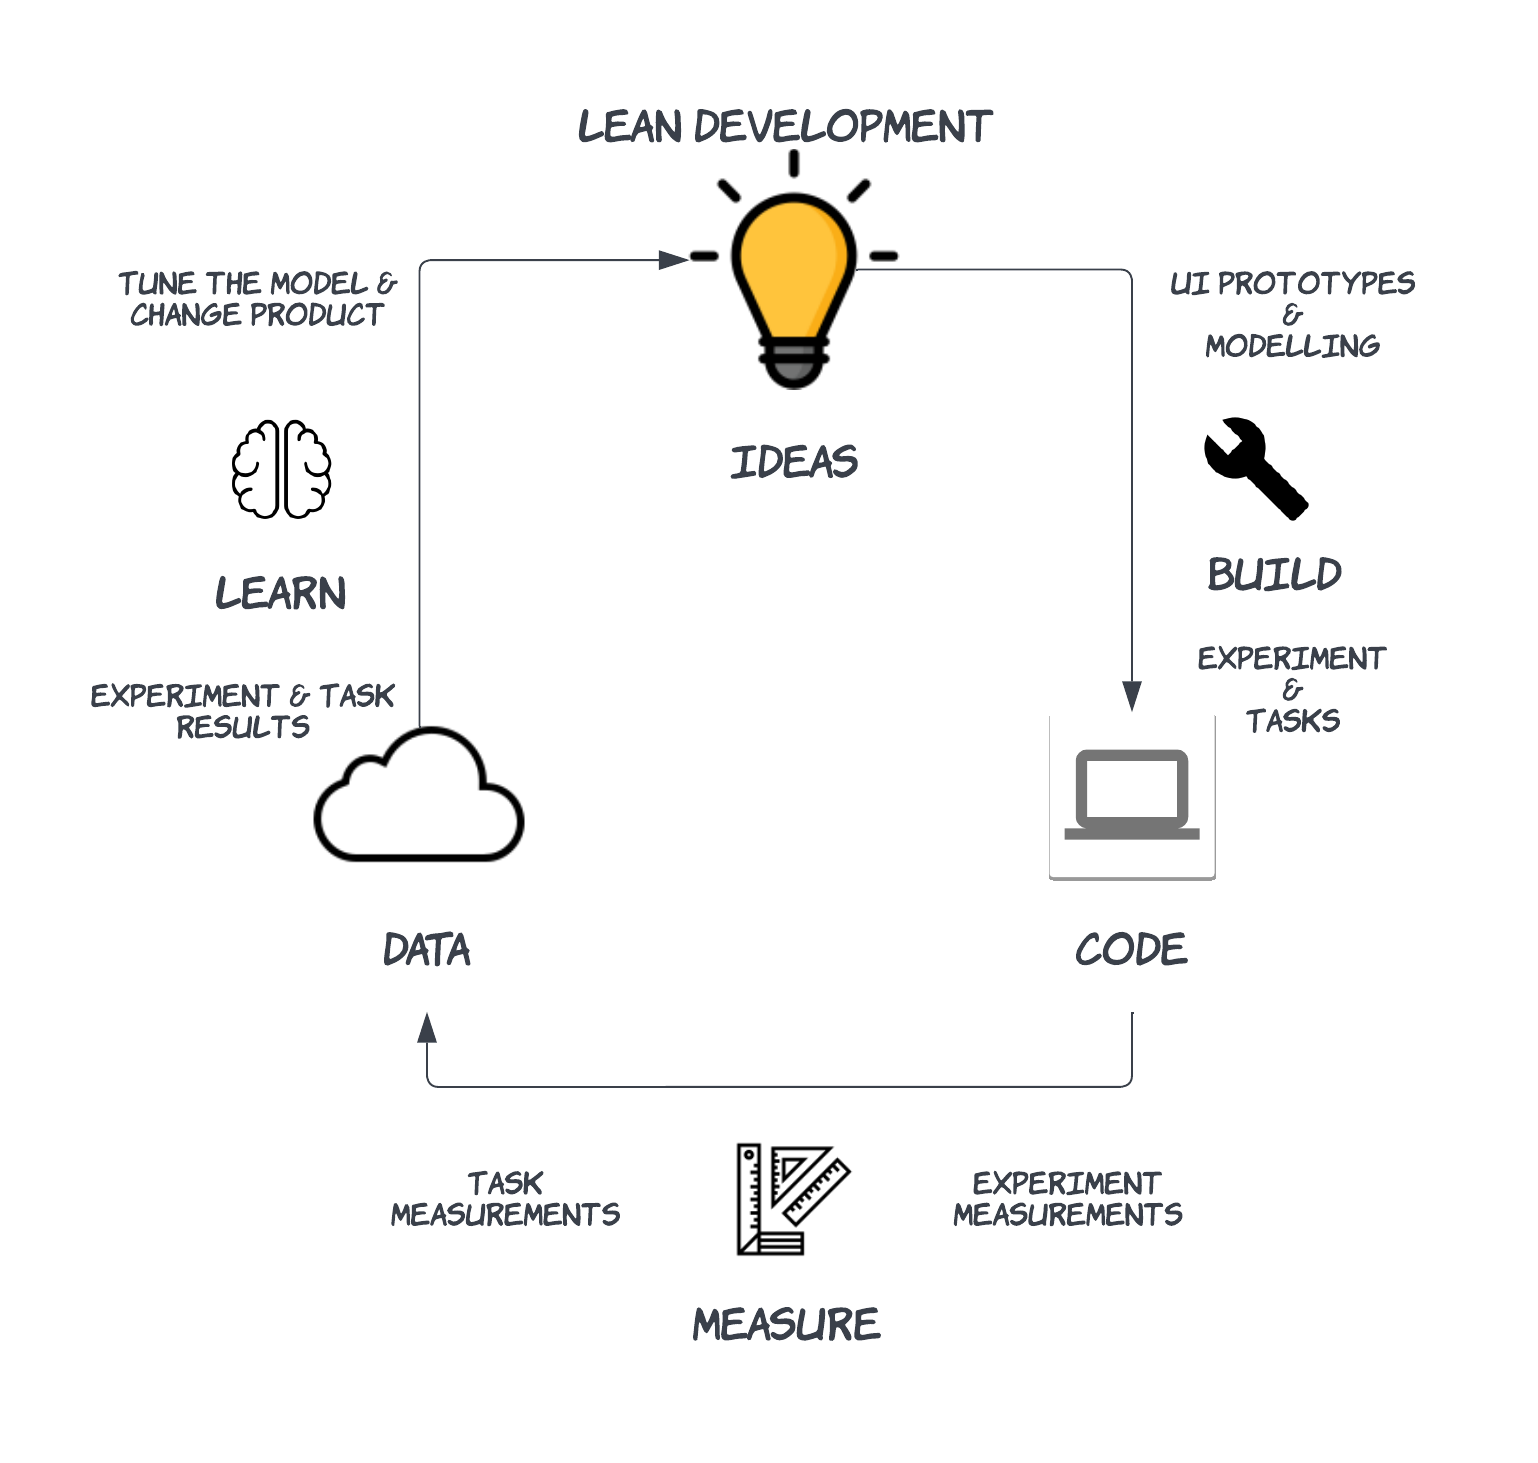
\includegraphics[scale=0.15]{images/solution-ideas/LEAN.png}
    \caption{LEAN Development technique}
    \label{intro:fig:lean}
\end{figure}
\par

\paragraph{Solution Approach:} In our solution, we use the LEAN development technique (see figure \ref{intro:fig:lean}) for development. LEAN development technique can be divided into 3 phases Build, Measure, and Learn. 
In the \texttt{(1) Build} phase, we plan to create the \texttt{UI Prototypes}, \texttt{Models}, create \texttt{Experiments}, and assign \texttt{Tasks} to the users. 
In the \texttt{(2) Measure} phase, we plan to measure the \texttt{Task and the Experiment measurements} and perform some analysis on the data received. 
And finally, in the \texttt{(3) Learn} phase, we display the \texttt{Experiment results}, \texttt{Tune} our models to decide the better variant among the others, and \texttt{Modify} our product. The solution approach is detailed in Chapter \ref{chap:solutionideas}.